\documentclass[11pt]{article}
%Gummi|063|=)
\title{\textbf{Cache Simulator Report}}
\author{Alok Hota, Mohammad Ahmadzadeh\\\href{https://github.com/auxiliary/CacheSimulator}{https://github.com/auxiliary/CacheSimulator}}

\usepackage{amsthm}
\usepackage{hyperref}
\usepackage{amsmath}
\usepackage{tikz}
\usepackage{graphicx}
%\usepackage{placeins}
%\setlength{\parindent}{0pt}
%\usepackage[margin=0.5in]{geometry}
\begin{document}

\maketitle

\section{Development}
\paragraph{}
Our cache simulator takes a configuration file and a trace file from the command line. It then generates a memory hierarchy based on the configurations and runs the instructions read from the trace file. 

\subsection{Features}
\paragraph{}
The following features have been implemented in the cache simulator:
\begin{itemize}
	\item Fully configurable cache hierarchy using YAML
		\begin{itemize}
			\item Architecture details, level 1 cache and main memory are required
			\item Level 2 and level 3 are optional
		\end{itemize}
	\item Supports write through and write back
	\item Optionally draws cache layout after simulation
	\item Writes simulation results to a log file and standard output
\end{itemize}

\subsection{Assumptions}
\begin{itemize}
	\item When a new word is written to level 1 cache, a new block is allocated. If the CPU then reads another word from that block it will be reading an empty word. The simulator will count this as a read hit. This would actually result in a segfault but we consider this out of scope. 
\end{itemize}

\subsection{Functionality}
\paragraph{}
The code begins with getting arguments from the command line using the argparse module and reads in cache configurations using the YAML format. The memory hierarchy is then created from the configurations. This is done using a bottom-up approach. We do this so that each level of cache can point to the previous level. The \textit{build\_hierarchy} function utilizes the \textit{Cache} class for each level. After setting up logging features the code reads the trace file given by the user and a starts the simulation. Optionally it draws the final contents of each cache after simulation. 

\paragraph{}
The constructor of the \textit{Cache} class takes every configurable parameter needed for the cache and creates an empty cache object. The data in the cache is represented by a Python dictionary structure. The top level keys are set indexes, each of which contains another dictionary keyed by ways. Every way's value is a Block object, which contains its own metadata, such as a \textit{dirty\_bit} and \textit{last\_accessed} time for LRU. 

\paragraph{}
The \textit{Cache} class contains \textit{read} and \textit{write} methods that are called during simulation. The following figures depict the overall structure of this process. Note that when writing to next level, we are calling the next cache's write method recursively. The same goes for reading from the next level and getting back the response. In addition, the \textit{read} method will call \textit{write} if a block is being replaced. 

\begin{figure}[htp!]
\centering
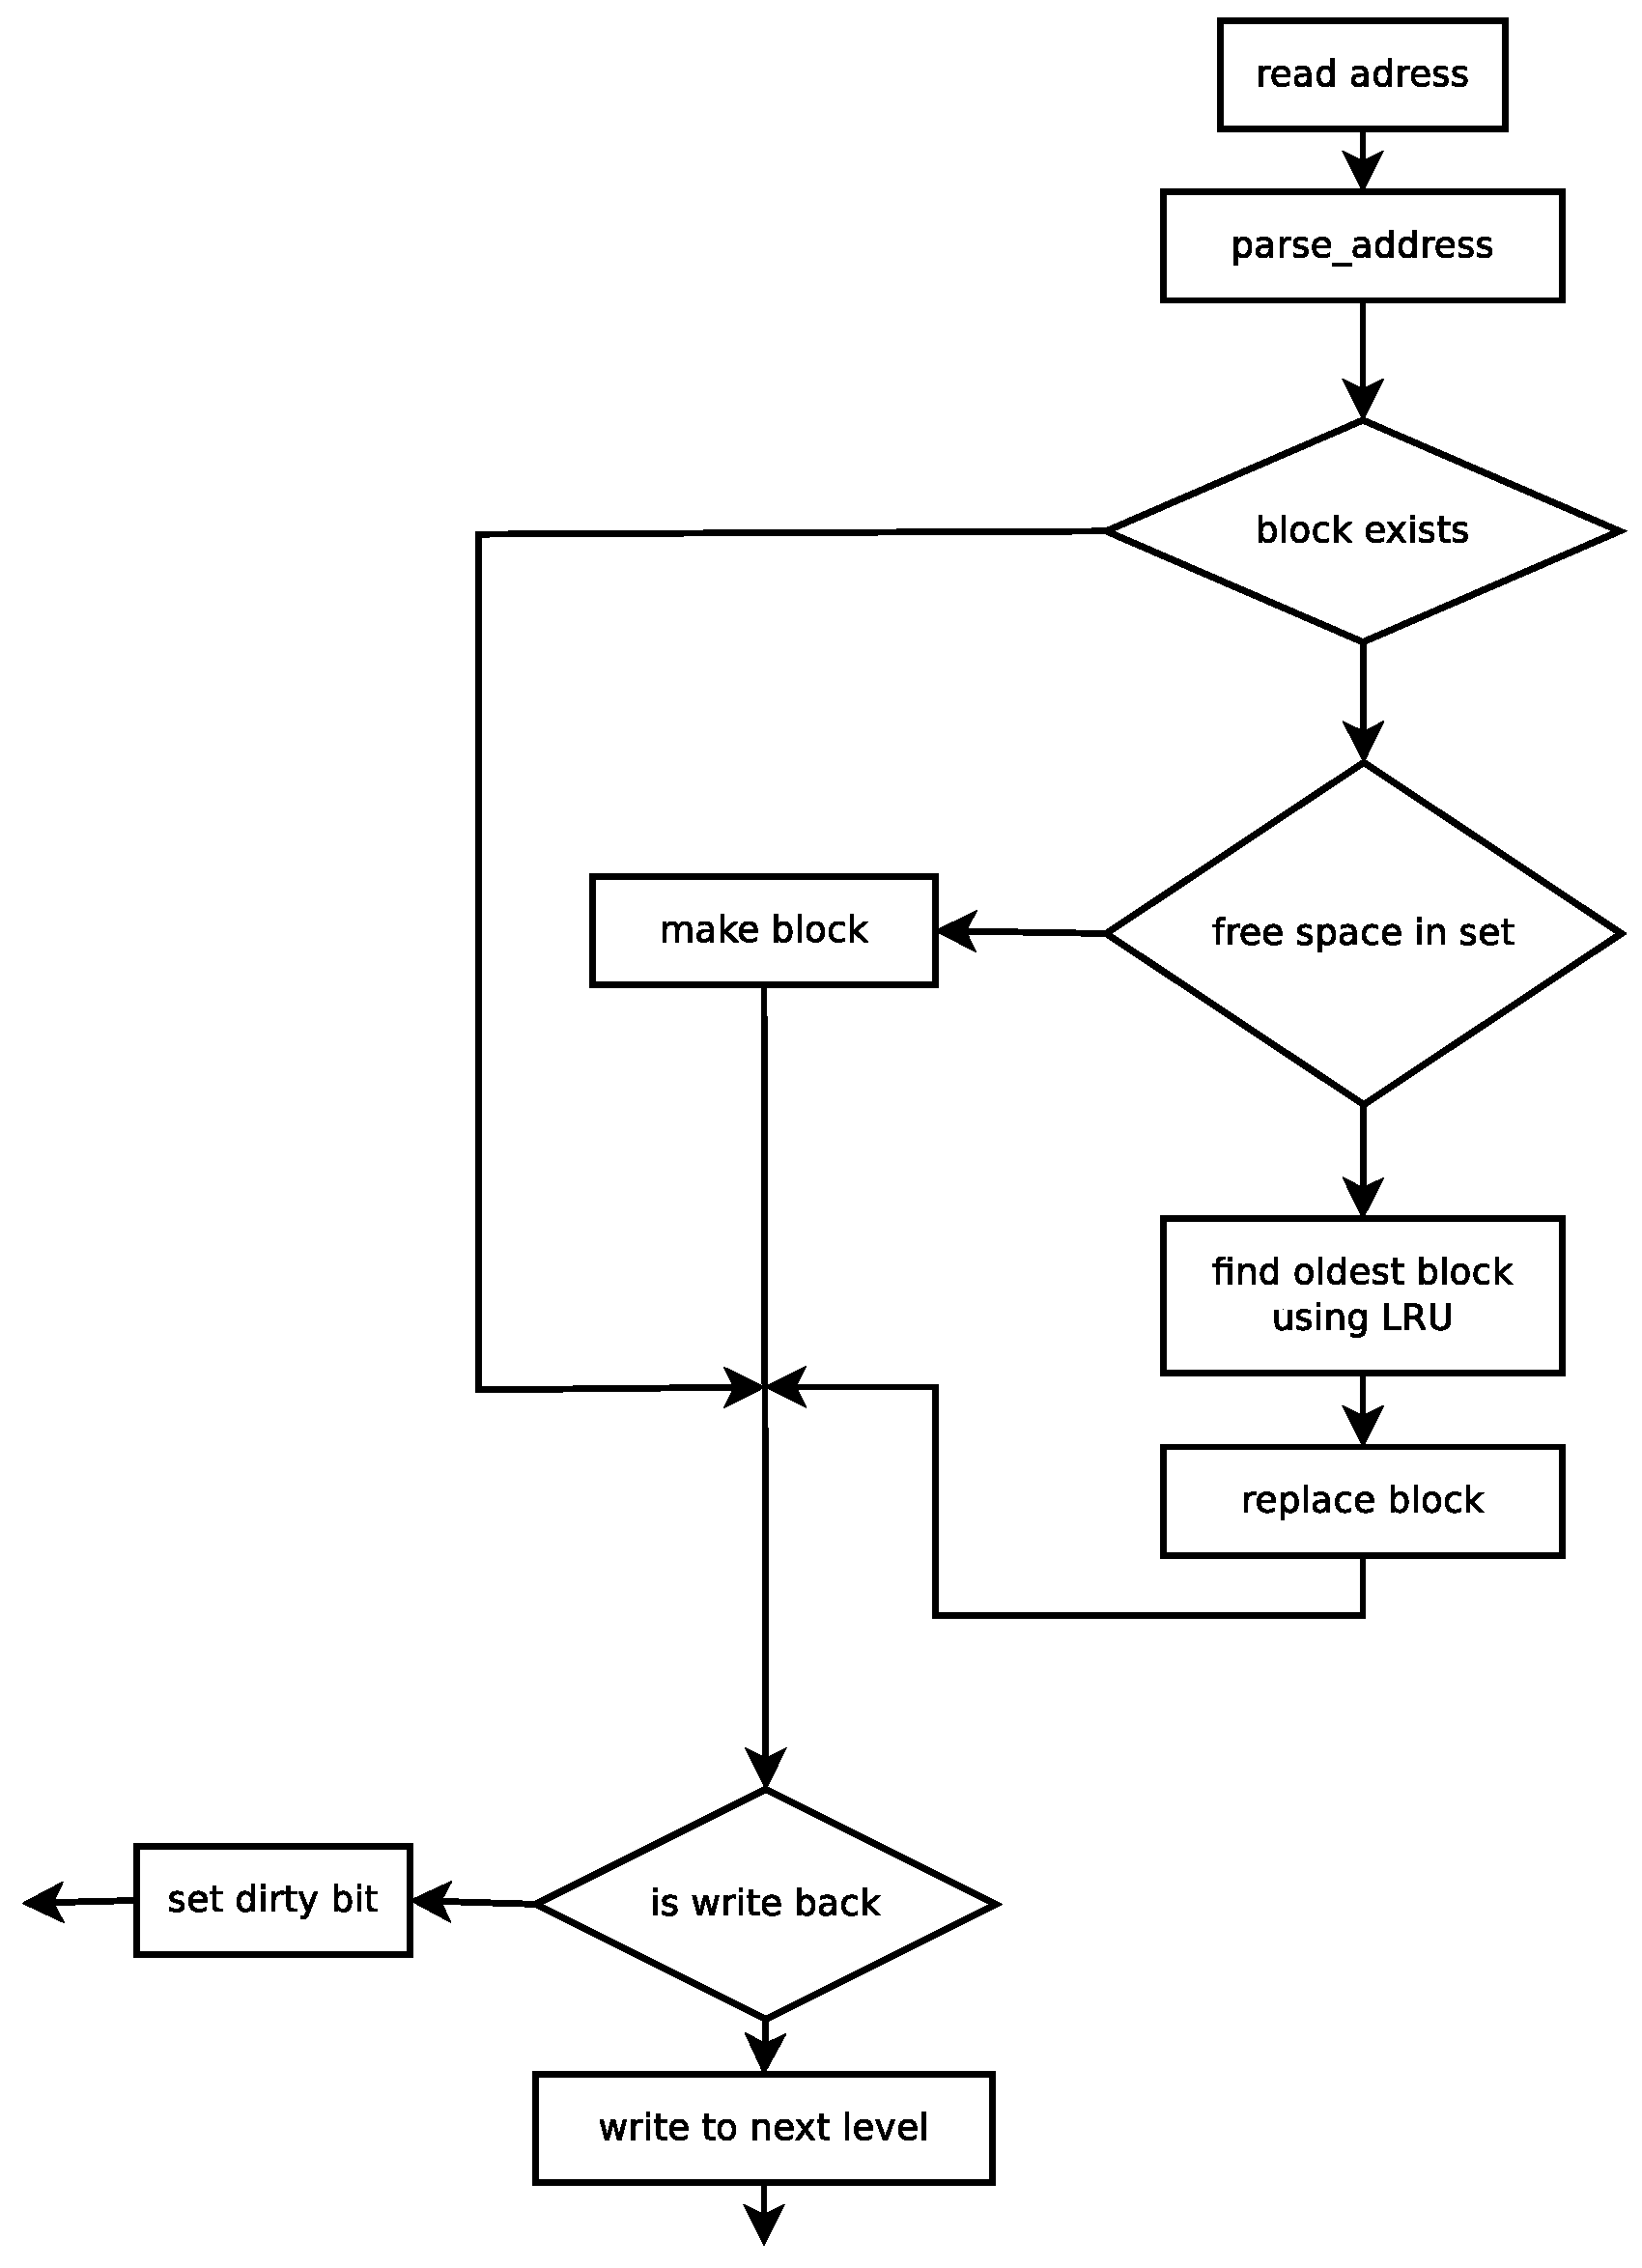
\includegraphics[scale=0.40]{write_diagram.eps}
\caption{Overview of workflow for writing an address to cache}
\label{}
\end{figure}

\begin{figure}[htp!]
\centering
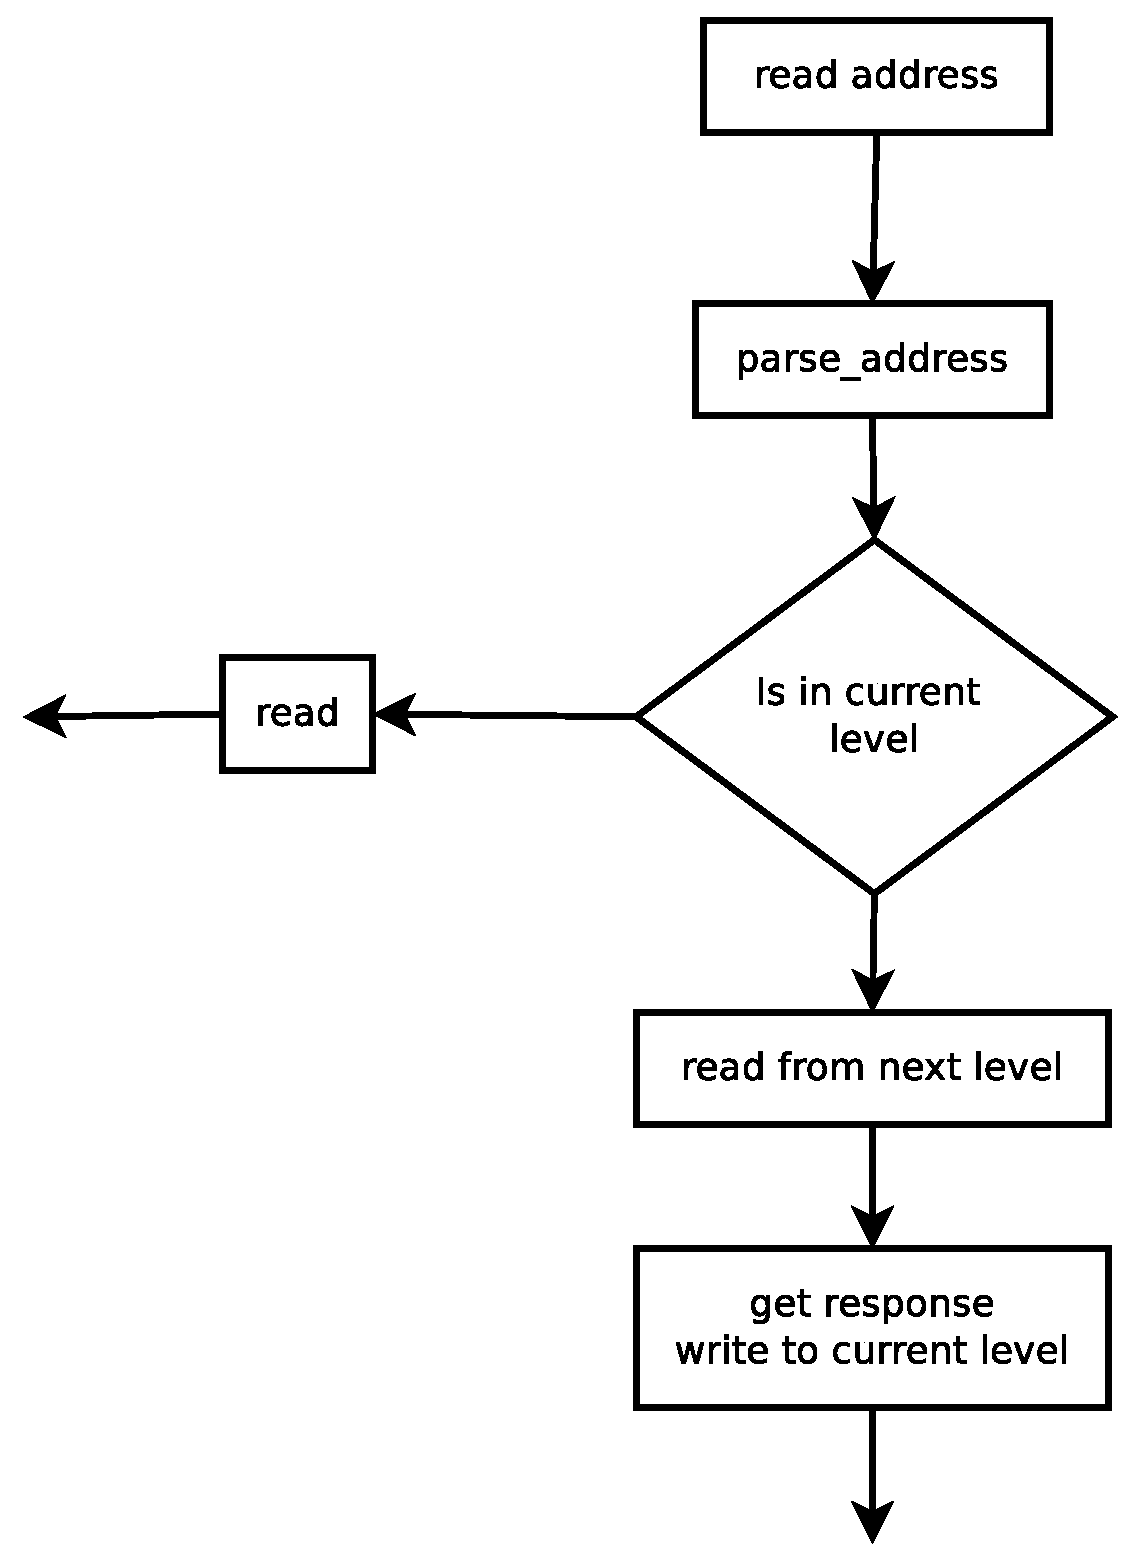
\includegraphics[scale=0.40]{read_diagram.eps}
\caption{Overview of workflow for reading an address from cache}
\label{}
\end{figure}

\pagebreak
\paragraph{}
The simulation and calculation of AMAT rely on the \textit{Response} objects. Response objects are created when an instruction is completed. They keep a record of the total time taken by the instruction and a trace of which levels of cache the instruction hit. 

\section{Testing}
\paragraph{}
We tested the simulator with several different cache configurations and trace files as well as a stress test. The stress test is generated with a python script located in gen\_test/gen\_stress\_test.py and provides a large randomly generated trace file. These random instructions very rarely result in a hit, which demonstrates the functionality of caches. If stress test is run with our \textit{config\_simple\_multilevel} configuration, the AMAT for L1 is 1117 cycles as opposed to 1000 for memory alone. This shows that having poor hit rate and write allocate leads to an 11\% increase in time taken. There are many other configurations and trace files included with which to test. 

\section{Conclusion}
\paragraph{}
Writing this simulator greatly inforced the concepts of sets, ways, write back, write through and write allocate. 

\end{document}
